\chapter{Project Plan}
\begin{figure}[h!]
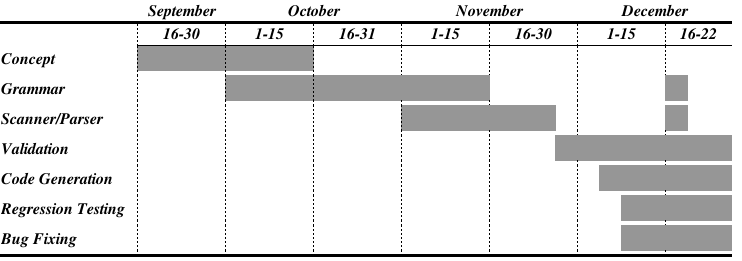
\includegraphics[scale=.5]{timeline.png}
\caption{Timeline for Setup Team}
\end{figure}

\textbf{September. } Our team held weekly meetings to discuss different potential ideas for a language.  By the end of the month, we had decided on a language that would manipulate sets.  We then set to work developing a rough draft for a working grammar and began drafting our reference manual.

\textbf{October. } In conjunction with writing the first draft of our LRM, we began work on the scanner and parser. As we built the parser, we found several areas where our grammar needed to be "improved."  The following graphic illustrates nicely how we spent October:

\tikzstyle{circ} = [circle, minimum height = 5em, minimum width = 5em, text centered, fill=blue!40, drop shadow, draw = blue]
\tikzstyle{toarrow} = [->, >= open triangle 90, thick]

\begin{center}
\begin{tikzpicture}
	\node (g) [circ] at (5,0) {Grammar};
	\node (s) [circ] at (7.5,-2.5) {Scanner};
	\node (p) [circ] at (2.5,-2.5) {Parser};
	
	\draw [toarrow] (g) -- (s) node [midway] {update};    
    \draw [toarrow] (s) -- (p) node [midway] {update};
    \draw [toarrow] (p) -- (g) node [midway] {update};
\end{tikzpicture}
\end{center}

\textbf{November. } We completed work on our parser in November and began working on validation (static semantic analysis) to perform type checking.  By the end of the month we were at the point where we could start generating code.

\textbf{December. } Writing code to generate valid C++ turned out to be more difficult than we anticipated, largely due to deep typing of nested tuples, and we continued to struggle with the Set-Builder construction mechanism.  We implemented a set class abstraction in C++ to handle some of the peculiarities of arbitrary set and tuple containers. Throughout December, we generated code and tested for bugs.

